\newpage
\appendix
\appendixpage
\addappheadtotoc

Important details such as the steps gone through were documented in \url{https://github.com/MinghongAlexXu/JetBot/tree/16de560ec3843861ca7abe4e7b711e4e5e5ece9d/note}.



\section{Interfacing sensors}

I2C Linux driver and drivers for DuPPa I2C Encoder Mini, LSM303D, and ICM20600 were implemented in C++. Unit test for each driver were also written.

\begin{figure}[htbp]
   \centering
   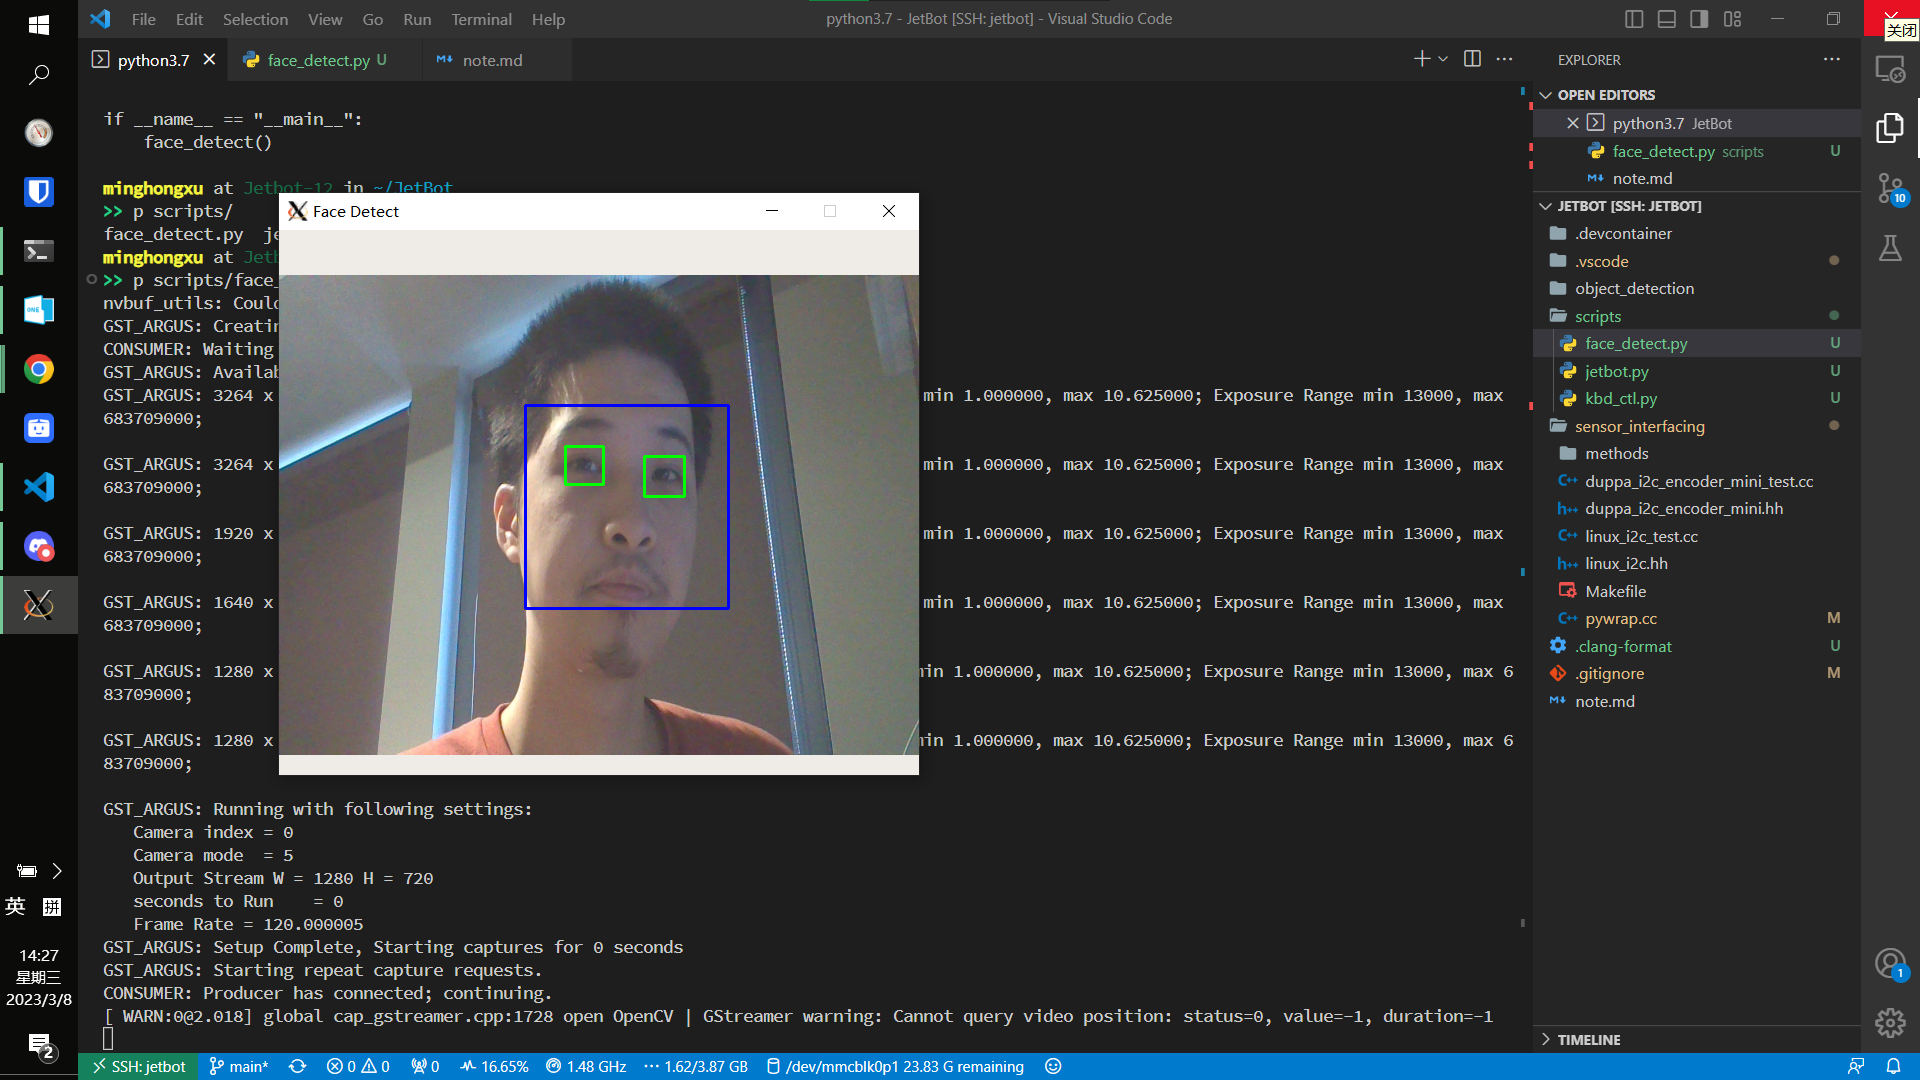
\includegraphics[width=0.9\textwidth]{face-detect}
   \caption{Testing the CSI camera}
   \label{fig:face-detect}
\end{figure}



\section{Lane marking following}

\begin{figure}[htbp]
\centering
\begin{subfigure}[b]{0.49\textwidth}
   \centering
   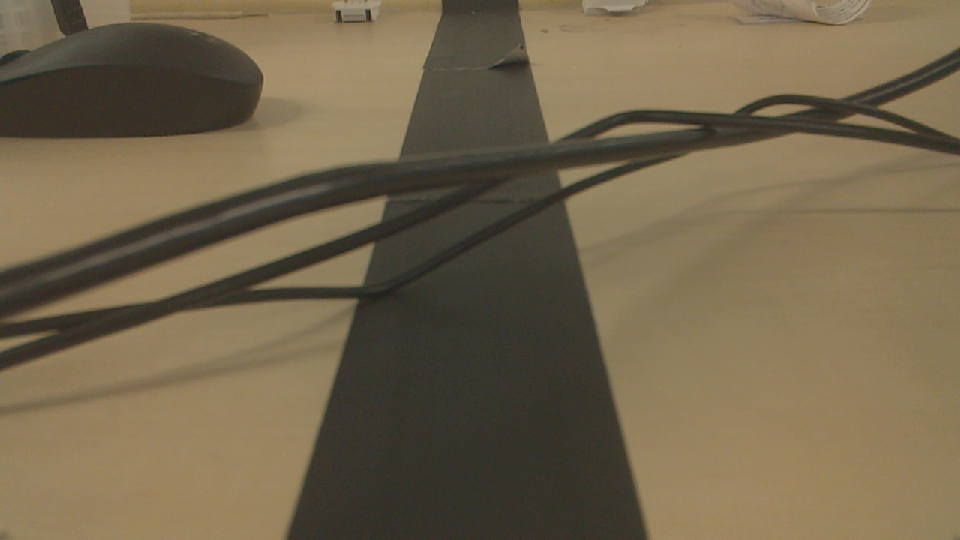
\includegraphics[width=\textwidth]{original-perspective}
   \caption{Original perspective}
\end{subfigure}
\begin{subfigure}[b]{0.49\textwidth}
   \centering
   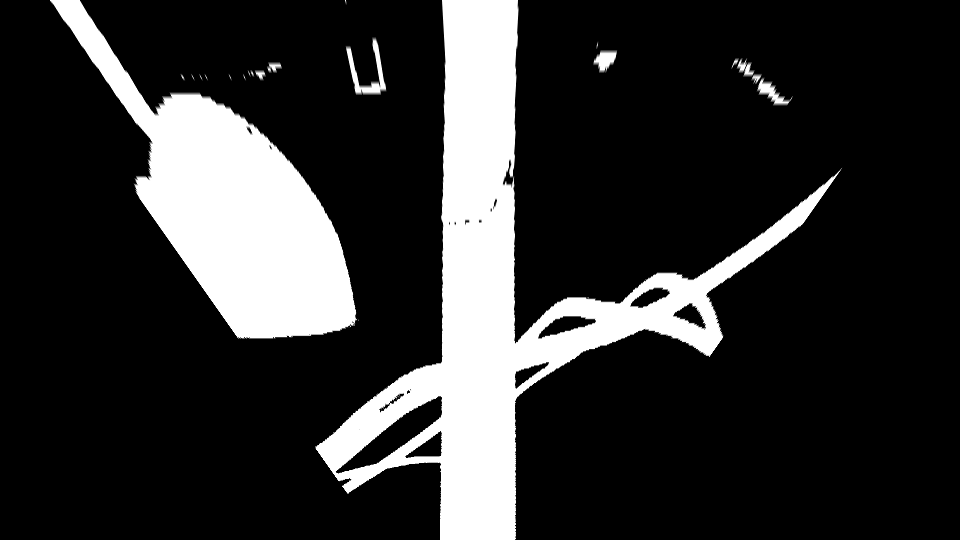
\includegraphics[width=\textwidth]{virtual-bird-view}
   \caption{Segmented and bird-view transformed}
\end{subfigure}
\caption{Image processing before fitting a parabola to the lane mark}
\label{fig:line}
\end{figure}


\newpage
\section{SLAM with Google Cartographer}

\begin{figure}[htbp]
   \centering
   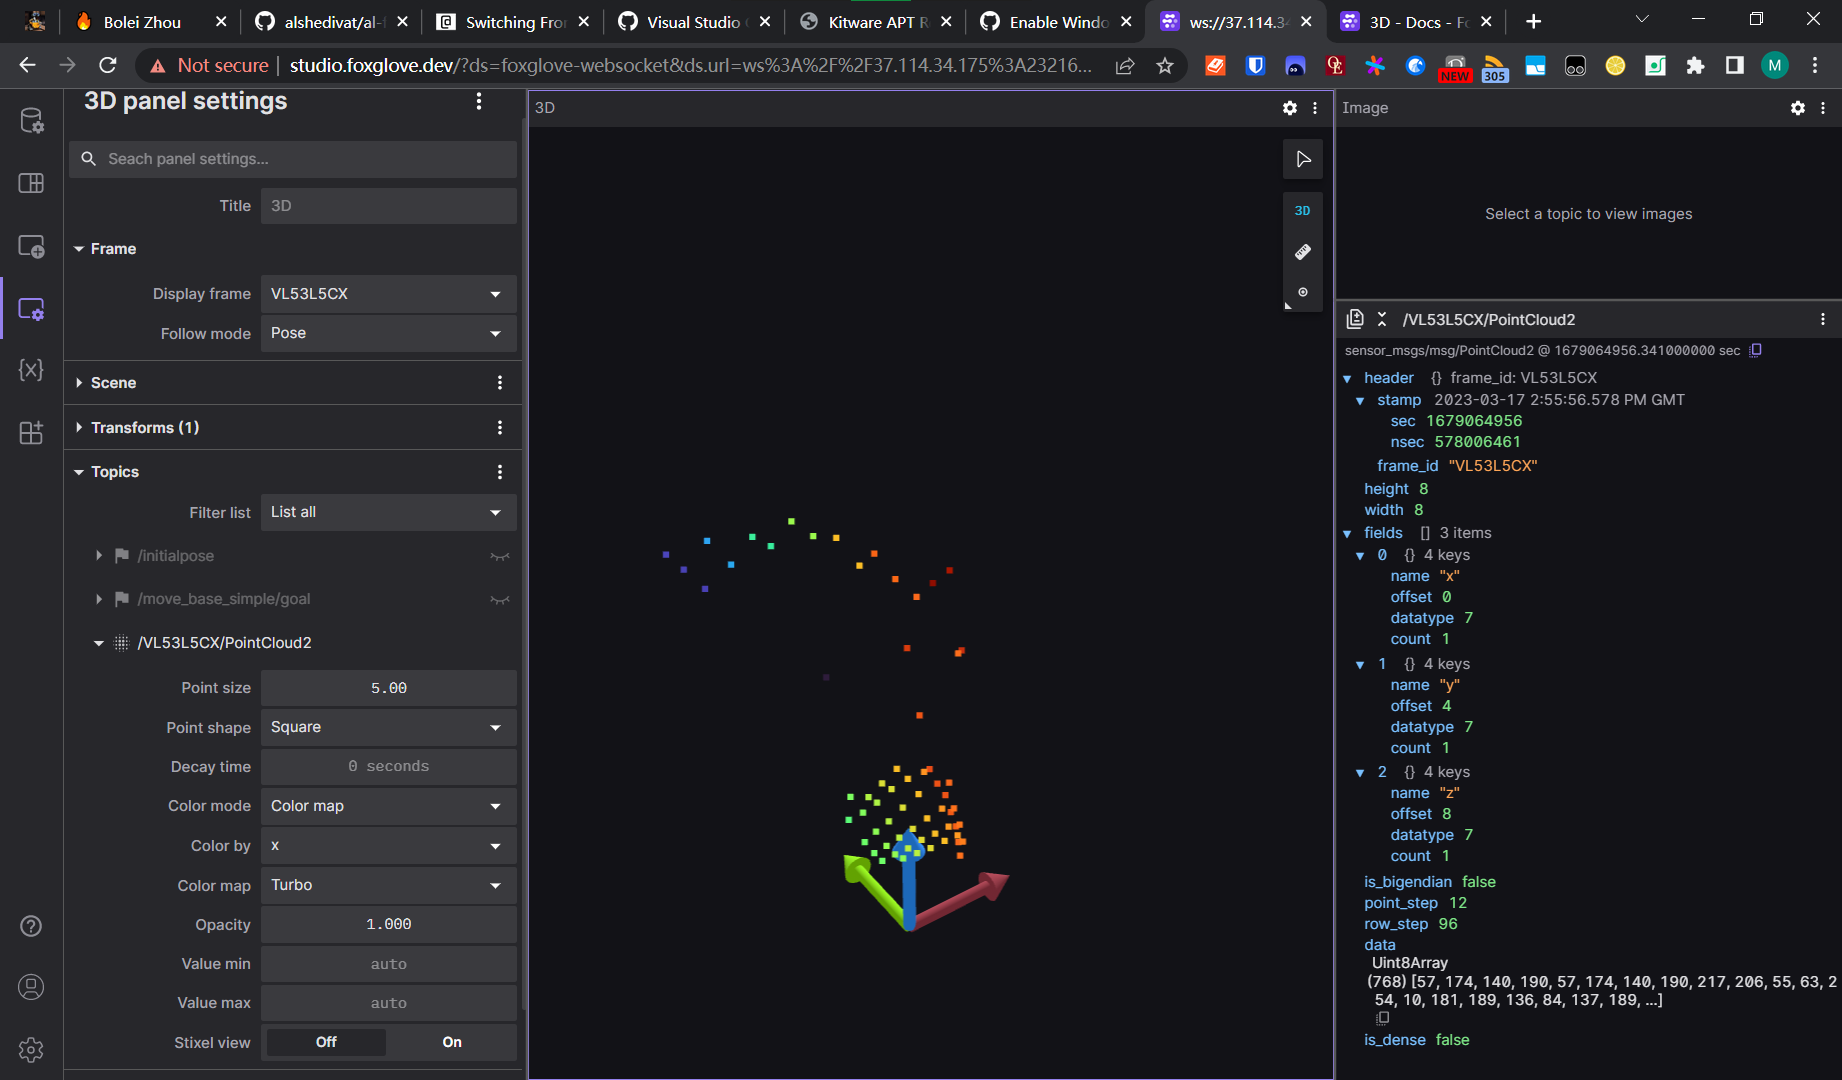
\includegraphics[width=0.87\textwidth]{vl53l5cx}
   \caption{VL53L5CX data visualised in Foxglove}
   \label{fig:vl53l5cx}
\end{figure}

\begin{figure}[htbp]
   \centering
   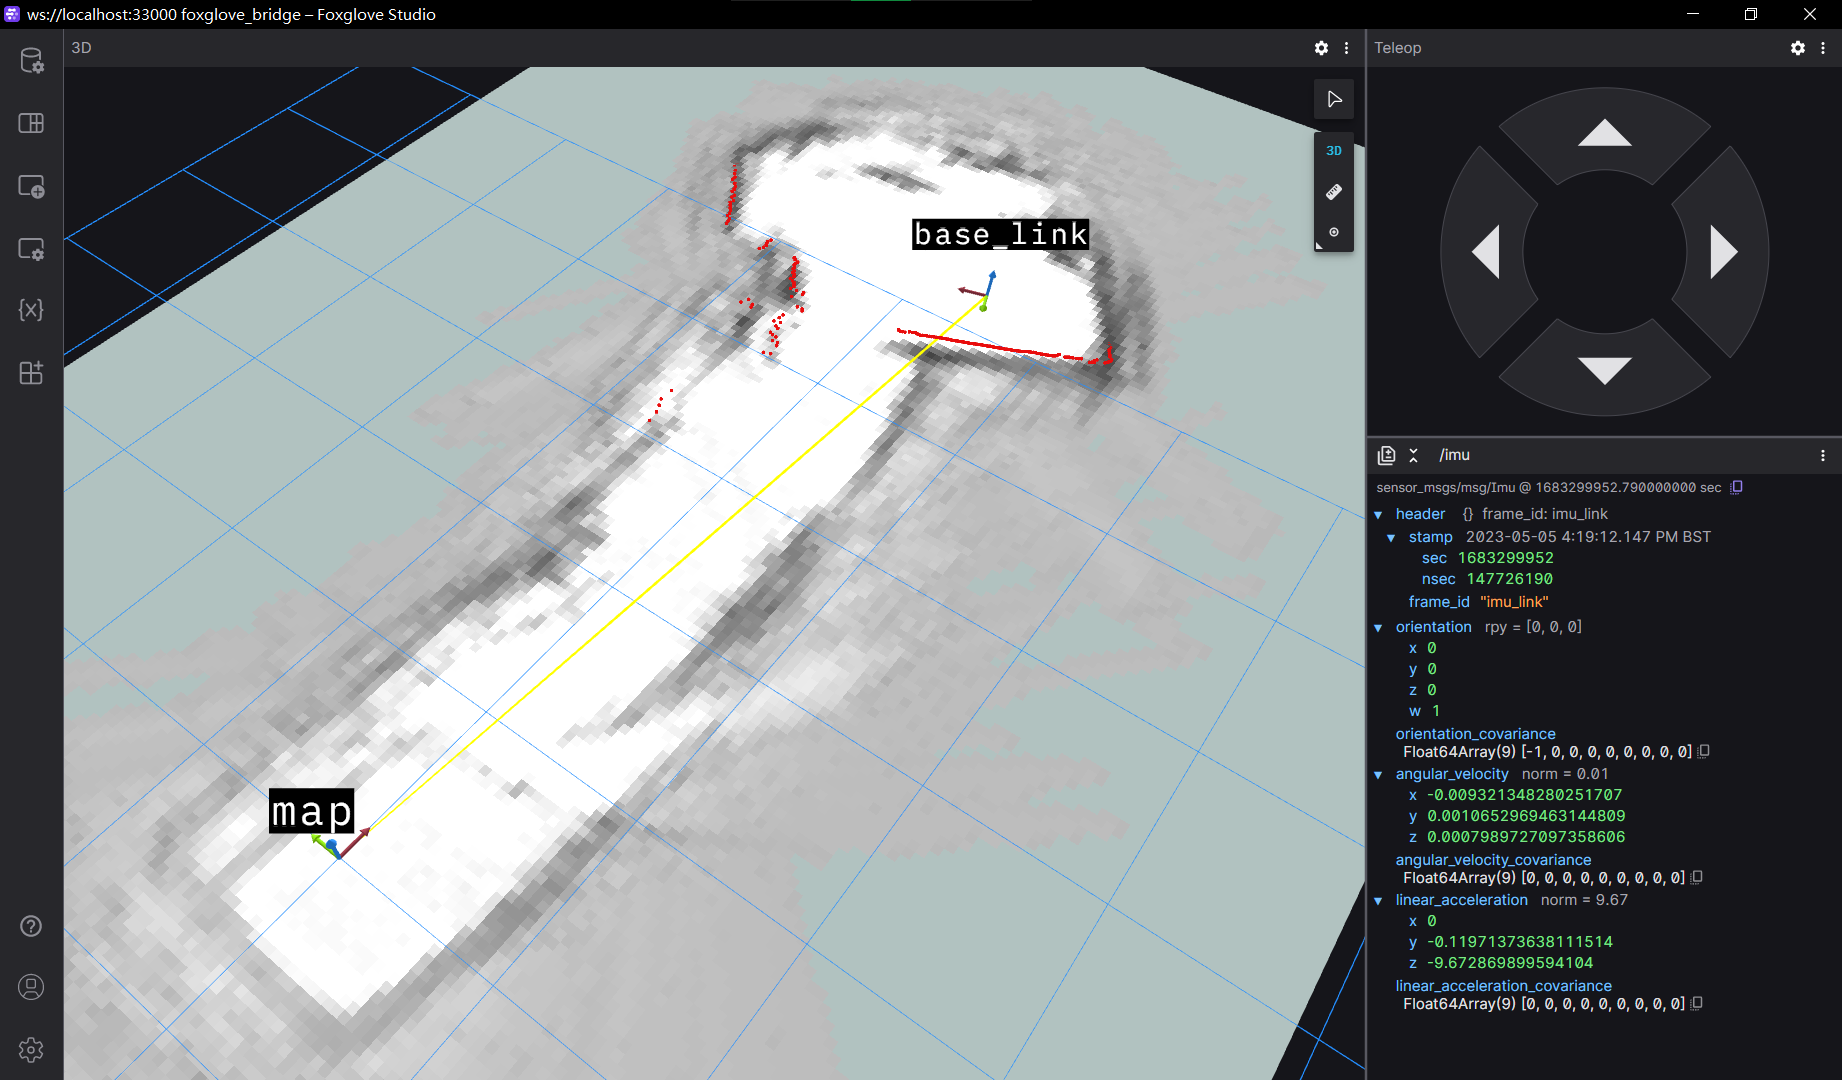
\includegraphics[width=0.87\textwidth]{cartographer}
   \caption{Map of a corridor with a 2D LiDAR}
   \label{fig:cartographer}
\end{figure}
